\documentclass{report}
     
    \usepackage{pgf,pgfplots}
     
    \usetikzlibrary{fit,calc}
    \usepgfplotslibrary{external}
     
    \newcommand{\boxplot}[6]{%
         %#1: center, #2: median, #3: 1/4 quartile, #4: 3/4 quartile, #5: min, #6: max
         \pgfmathparse{#1+0.25}\edef\boxxr{\pgfmathresult}%
         \pgfmathparse{#1-0.25}\edef\boxxl{\pgfmathresult}%
         \pgfmathparse{#1+0.15}\edef\whiskerr{\pgfmathresult}%
         \pgfmathparse{#1-0.15}\edef\whiskerl{\pgfmathresult}%
         \filldraw[fill=green!20,line width=0.2mm] (axis cs:\boxxl,#3) rectangle (axis cs:\boxxr,#4);% draw the box
         \draw[line width=0.2mm, color=red] (axis cs:\boxxl,#2) -- (axis cs:\boxxr,#2);              % median
         \draw[line width=0.2mm] (axis cs:#1,#4) -- (axis cs:#1,#6);                                 % bar up
         \draw[line width=0.2mm] (axis cs:\whiskerl,#6) -- (axis cs:\whiskerr,#6);                   % upper quartile
         \draw[line width=0.2mm] (axis cs:#1,#3) -- (axis cs:#1,#5);                                 % bar down
         \draw[line width=0.2mm] (axis cs:\whiskerl,#5) -- (axis cs:\whiskerr,#5);                   % lower quartile
    }
     
    \begin{document}
     
    \tikzset{external/remake next}
    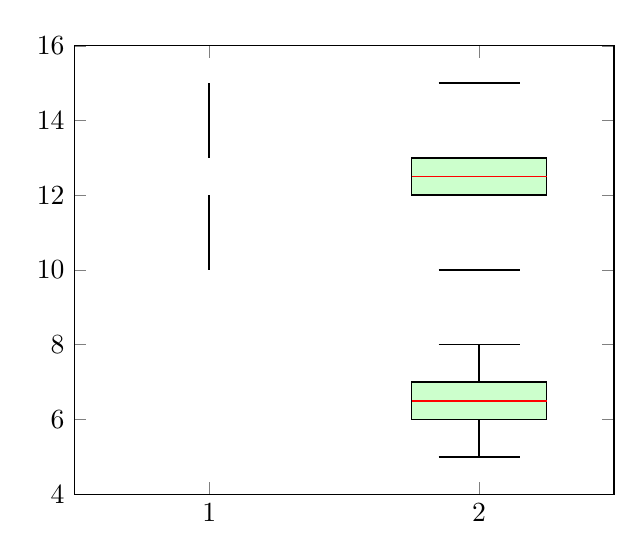
\begin{tikzpicture}
    \begin{axis}[xmin=0.5, xmax=2.5, ymin=4, ymax=16,
                  xtick={1,2},
                  xticklabels={1,2}]
    %#1: center, #2: median, #3: 1/4 quartile, #4: 3/4 quartile, #5: min, #6: max
    \boxplot{1}{12.5}{12}{13}{10}{15}
    \boxplot{2}{6.5}{6}{7}{5}{8}
    \end{axis}
    \end{tikzpicture}
     
    \end{document} 
